\documentclass[12pt]{article}

\usepackage[margin=1in]{geometry}
\usepackage[british]{babel}
\usepackage[style=american]{csquotes}
\usepackage{orcidlink}
\usepackage{fontspec}
\setmainfont{Charis SIL} % compile with LuaLaTeX or XeLaTeX
\usepackage[final]{microtype}
\usepackage{marvosym}
\usepackage{enumitem}
\usepackage{hyperref}
\hypersetup{
    colorlinks=true,
    linkcolor=blue,
    citecolor=blue,
    pdfauthor={Brett Reynolds},
    pdftitle={Naturalizing Typological Kinds: Comparanda, Mechanisms, and Measurement}
}

\usepackage{amssymb,amsmath}
\usepackage{graphicx}
\usepackage{langsci-gb4e}

\usepackage{array,booktabs} % booktabs optional but recommended
\newcolumntype{L}[1]{>{\raggedright\arraybackslash}p{#1}}


\usepackage[style=apa,backend=biber]{biblatex}
\DeclareLanguageMapping{british}{british-apa}
\addbibresource{references.bib}

% House style macros
\newcommand{\term}[1]{\textit{#1}}

\title{Naturalizing Typological Kinds:\\Comparanda, Mechanisms, and Measurement}
\author{Brett Reynolds \orcidlink{0000-0003-0073-7195}\thanks{I used ChatGPT 5, Claude Sonnet 4.5, and Gemini Pro 2.5 extensively in drafting and revising the paper. I reviewed, edited, and approved all the material and take full responsibility for the final text and conclusions. \href{mailto:brett.reynolds@humber.ca}{brett.reynolds@humber.ca}}\\Humber Polytechnic \& University of Toronto}
\date{\today}


\begin{document}
\maketitle


\begin{abstract}
Typological universals often dissolve because analysts collapse language-internal categories with the cross-linguistic comparanda they are meant to instantiate. When English \textsc{noun}\textsubscript{Eng} or Hebrew \textsc{subject}\textsubscript{Heb} is projected directly onto a purportedly universal \textsc{noun}\textsubscript{\Cross}, measurement error and spurious asymmetries accumulate.

I propose a homeostatic framework that keeps the levels apart and makes the explanatory work accountable. First, a three-tier \emph{comparanda--realization} mapping separates cross-linguistic functions, semantic targets, discourse roles, and categories from their language-specific realizations. Second, a \emph{syntax--semantics hygiene} protocol diagnoses targets independently of morphosyntactic exponents, ensuring that comparative concepts travel without dragging language-particular packaging. Third, some comparanda earn promotion to \emph{naturalized comparative concepts} when convergent cognitive, discourse, diachronic, or community mechanisms maintain their property clusters; others are tagged with explicit failure modes.

The framework issues risk-bearing predictions about trade-offs, regeneration pathways, and latent-variable diagnostics (e.g., \emph{nominality}) and is formalized in an auditable specification (\texttt{src/typology.py}). By demanding mechanisms as well as mappings, the account preserves the empirical ambition of typology while avoiding the universalist overreach that has long haunted the field.
\end{abstract}

\section{Orientation}\label{sec:orientation}
Two requirements conflict: cross-linguistic comparison needs predicates that travel across grammars, while grammatical analysis needs kinds that are grammar-specific. From this tension, typology accumulates measurement error and fragile generalizations.

I adopt a terminological discipline following \textcite{HuddlestonPullum2002}: \emph{function} (unqualified) denotes syntactic functions only; \emph{target} denotes semantic targets; \emph{role} denotes discourse/pragmatic roles; \emph{category} denotes syntactic categories. Subscripts distinguish comparative cross-linguistic concepts (\textsc{term}\textsubscript{\Cross}) from language-specific realizations (\textsc{term}\textsubscript{Eng}, \textsc{term}\textsubscript{Jpn}) and general language-internal references (\textsc{term}\textsubscript{$L$}) where no particular language is in focus.

Following \textcite{Haspelmath2010}, I treat cross-language targets as \emph{comparative concepts}~-- analyst-constructed categories that allow comparison without assuming the categories exist in individual grammars. Building on \textcite{Croft2001,HuddlestonPullum2002}, I analyse language-internal lexical categories as homeostatic property cluster (HPC) kinds~-- categories that persist because mechanisms maintain clustered properties, not because they have essential defining features \parencite{Boyd1991Enthusiasm,Boyd1999Homeostasis,Khalidi2013}. I call these cross-linguistic targets \emph{comparanda}~-- the phenomena we compare across languages, distinct from language-specific realizations.

The foundation: clear descriptions of language-internal syntactic categories and functions~-- English's noun, Japanese's relative clause, Hebrew's subject~-- with their full morphosyntactic property clusters. Cross-linguistic comparison then requires apparatus that permits asking whether English's noun and Japanese's noun realize similar patterns, without presupposing that English's cluster defines the universal or that cross-linguistic prototypes have to mirror any particular realization. Section~\ref{sec:failures} details how systematic conflation errors block this goal.


Table~\ref{tab:levels} presents the three-level ontology that separates what we compare across languages from what exists in particular grammars.

\begin{table}[ht]
  \centering
  \caption{Three-level ontology for comparative concepts and realizations}\label{tab:levels}
  \begin{tabular}{p{3cm}p{6.2cm}p{5.5cm}}
    \toprule
    Level & Contents & Diagnostic focus \\
    \midrule
    Level-I: \hspace{1.5cm} cross-linguistic pressures & Semantic targets (\textsc{specificity}\textsubscript{\Cross}, \textsc{definiteness}\textsubscript{\Cross}, \textsc{mass/count}\textsubscript{\Cross}) and discourse roles (\textsc{topic}\textsubscript{\Cross}, \textsc{focus}\textsubscript{\Cross}, \textsc{vocative}\textsubscript{\Cross}) & Behavioural tests on interpretation, common ground management, and discourse continuity \\ \addlinespace[4pt]
Level-II: \hspace{1.5cm} cross-linguistic syntax & Functions (\textsc{subject}\textsubscript{\Cross}, \textsc{head}\textsubscript{\Cross}, \textsc{predicate}\textsubscript{\Cross}) and categories (\textsc{V}\textsubscript{\Cross}, \textsc{VP}\textsubscript{\Cross}, \textsc{clause}\textsubscript{\Cross}) & Portable morphosyntactic diagnostics (alignment, extraction, agreement control, slot privileges) \\ \addlinespace[4pt]
Level-III: language-internal syntax & Language-internal functions (\textsc{subject}\textsubscript{Eng}, \textsc{head}\textsubscript{Spn}, \textsc{predicate}\textsubscript{Tha}) and categories (\textsc{V}\textsubscript{Eng}, \textsc{VP}\textsubscript{Mndr}, \textsc{clause}\textsubscript{Hbr}) & Distributional, morphological, and prosodic evidence specific to $L$; mapped to Level~II with graded weights \\ \addlinespace[4pt]
    \bottomrule
  \end{tabular}
\end{table}

Multiple levels may converge in a single expression. In [\textit{the cat}] \textit{awoke}, the bracketed NP instantiates \textsc{topic}\textsubscript{\Cross} (Level~I) and \textsc{subject}\textsubscript{\Cross} (Level~II) via the language-internal function \textsc{subject}\textsubscript{Eng} (Level~III).

Levels~I and~III persist as homeostatic property-cluster kinds sustained by different mechanisms: cognitive–interactional pressures stabilize Level~I, while community-internal morphosyntax and diachrony sustain Level~III. Level-II comparanda , by contrast, are analyst-proposed comparative concepts. Some may earn \emph{naturalized} status (Section~\ref{subsec:naturalization-criteria}) and be treated (defeasibly) as kinds; others remain instrumental comparanda without ontological commitment.

Three additions operationalize this framework: an executable three-level \emph{comparanda--realization} schema (Section~\ref{sec:matrix}) separating what we compare (categories\textsubscript{\Cross}, functions\textsubscript{\Cross}, targets\textsubscript{\Cross}, roles\textsubscript{\Cross}) from what exists in particular languages (language-specific category realizations); an explicit \emph{syntax--semantics hygiene protocol} (Section~\ref{sec:hygiene}) testing semantic targets independently of their morphological or syntactic expression; and a measurement-first approach (Sections~\ref{sec:naturalized} and \ref{sec:measurement}) promoting some comparative concepts to \emph{naturalized} status when they show consistent cross-linguistic stability with identifiable homeostatic mechanisms.\footnote{A parallel object-oriented specification of these structures is maintained in \texttt{src/typology.py} to keep the theoretical machinery auditable.}

The paper proceeds as follows. Section~\ref{sec:failures} diagnoses four recurrent conflation errors in current typological practice, showing how they manifest in published research. Section~\ref{sec:matrix} operationalizes the three-level mapping with formal apparatus (mapping functions, weight assignment, reliability scores). Section~\ref{sec:hygiene} extends the framework to semantic targets through a hygiene protocol with operational diagnostics. Sections~\ref{sec:naturalized} and \ref{subsec:mechanisms} introduce naturalized comparative concepts and the homeostatic mechanisms that stabilize them, with a biological interlude (Section~\ref{sec:eyes}) illustrating character-identity mechanisms. Section~\ref{sec:measurement} develops measurement models using latent variables. Section~\ref{sec:predictions} derives five falsifiable predictions with declared thresholds. Section~\ref{sec:illustrations} applies the framework to three typological debates. Section~\ref{sec:threats} addresses objections about measurement feasibility, falsifiability, and circularity.

\section{Where typology goes wrong}\label{sec:failures}
Systematic errors in published typological research trace to a single source: conflating comparanda (categories\textsubscript{\Cross}, functions\textsubscript{\Cross}, targets\textsubscript{\Cross}, roles\textsubscript{\Cross}) with language-internal categories\textsubscript{$L$} and $L$-functions, or meanings with forms. The confusions run bidirectionally~-- language-internal categories project onto comparative functions and vice versa; property clusters of local realizations project onto comparative notions and vice versa~-- generating four recurrent obstacles.

\subsection{Four obstacles manifested}\label{subsec:failure-modes}

\emph{Dual-use terminology and category--function conflation} (obstacle a) arises when the same label is pressed into service for different ontological levels, encouraging analysts (or readers) to treat unlike phenomena as identical. A textbook example is \term{determiner}: it often names an NP-internal syntactic function and, at the same time, the lexical category realized in English by words like \textit{the}, \textit{this}, \textit{many}.  \textcite{Reynolds2025Definiteness} has recently pointed out that \textit{definite} is used as both a semantic term and for the exponent that prototypically realize definite semantics. \textit{Adverb}(\textit{ial}) commonly confounds adjuncts in general with a lexical category that commonly functions as adjuncts. \textit{Topic} is used multiply for categories (e.g., \textit{topic marker}), a discourse/pragmatic role, and prosodic/intonational patterns. Although many linguists and laypeople are aware of this polysemy and try to guard against it, confusion abounds. Maintaining strict terminological hygiene is best practice, even if that means creating vulgar neologisms.

\emph{Cluster reduction} (obstacle b) collapses a syntactic category's rich morphosyntactic property profile~-- distributional privileges, paradigmatic contrasts, agreement patterns, extraction behaviour~-- into a few semantic or discourse-functional properties; treating nouns as \enquote{thing-words} or subjects as \enquote{agents} discards the morphosyntactic evidence that defines these categories within their grammars.

\emph{Template import} (obstacle c) projects one language's morphosyntactic profile onto cross-linguistic prototypes: defining \textsc{subject}\textsubscript{\Cross} by properties of a particular category profile (nominative NP controlling agreement) bakes English or Russian structure into the comparative concept, producing tautologies (nominative languages trivially \enquote{have subjects}) or spurious counterexamples (ergative systems \enquote{lack subjects}) \parencite{Dryer1997,EvansLevinson2009}.

\emph{False universalisation} (obstacle d) assumes that every language must realise cross-linguistic prototypes with similar formal properties, generating undergeneralisation (\enquote{no adjectives $ \Rightarrow$ no property modification}) or overprojection (\enquote{no determiners $\Rightarrow$ no definiteness}). Yet functions and targets persist where their prototypical categories are absent: the \textsc{modifier}\textsubscript{\Cross} function survives via relative clauses, property nouns, or participles where \textsc{adjective}\textsubscript{$L$} categories are absent \parencite{Dixon2010,Croft2001}; the \textsc{definiteness}\textsubscript{\Cross} target persists via demonstratives, possessive frames, or classifier complexes where \textsc{determinative}\textsubscript{$L$} categories are absent. A related error conflates semantic or discourse targets with morphosyntactic exponents: \textsc{definiteness}\textsubscript{\Cross} becomes synonymous with articles, \textsc{specificity}\textsubscript{\Cross} with accusative case, \textsc{agentivity}\textsubscript{\Cross} with subjecthood. Reported \enquote{universals} then track \emph{exponents} rather than \emph{targets}, misdiagnosing languages that lack the exponent as lacking the target.

\subsection{Concrete illustrations}\label{subsec:compressed}

\begin{exe}
\ex\label{ex:determiner-double-duty}
\textbf{Category–function conflation: \textsc{determiner} (function) vs.~\textsc{determinative} (category).}
\textcite{QuirkEtAl1972} use \emph{determiner} for both an NP-internal \emph{function} and a lexical \emph{category} (words like \textit{the}, \textit{many}, \textit{which}, \textit{each}). The conflation arises because the prototypical determinative\textsubscript{Eng} realizes the determiner\textsubscript{Eng} function, but determinatives\textsubscript{Eng} also function as modifiers\textsubscript{Eng} (e.g., \textit{the }[\textit{many}]\textit{ books that we have}) while phrases of other categories\textsubscript{Eng} may realize determiner\textsubscript{Eng} function (e.g., the genitive NP\textsubscript{Eng} in [\textit{June's}] \textit{shoe}).

The distinction between what something is (\textsc{determinative}\textsubscript{Eng} category) and how it relates to other constituents (\textsc{determiner}\textsubscript{Eng} function) disappears. Cross-linguistic projection generates confusion: does Japanese \enquote{have determiners}? Without specifying whether we're asking about a lexical category or a syntactic function, the question is unanswerable.

\ex\label{ex:definiteness-vs-articlehood}
\textbf{Cluster reduction: \textsc{definiteness}\textsubscript{\Cross} (semantic target) vs.\ article systems (morphosyntactic category).}
Large typological surveys proxy \textsc{definiteness}\textsubscript{\Cross} by article presence: WALS 37A and APiCS chapter~28 code languages as \enquote{having definiteness} only if they grammaticalize dedicated definite articles \parencite{Dryer2013WALSDefArt,APiCS2013DefArticles}. Some analyses treat articleless systems as lacking presuppositional definiteness altogether \parencite{SimikDemian2020}. But  \textsc{definiteness}\textsubscript{\Cross}~-- identifiability via anaphoric uptake, uniqueness inferences, familiarity presuppositions~-- is a semantic target maintained by discourse-pragmatic mechanisms (common ground management, bridging, topic continuity), while article systems are morphosyntactic categories maintained by grammaticalization, acquisition, and community transmission. Though grammaticalization conventionalizes their pairing, systematic dissociation nevertheless occurs \parencite{Reynolds2025Definiteness}. Articles\textsubscript{Eng} prototypically signal \textsc{definiteness}\textsubscript{\Cross} in familiar European languages, but this correlation is a local fact, not a definitional requirement.

Cross-linguistic projection generates undergeneralization: languages without articles are misdiagnosed as lacking \textsc{definiteness}\textsubscript{\Cross} altogether, collapsing a rich semantic target into the presence of a single morphosyntactic exponent. Yet definiteness diagnostics~-- anaphora, uniqueness, anti-novelty contexts~-- still apply in articleless languages \parencite{Lyons1999,Matthewson2004}. Even English shows systematic divergences: weak definites (\textit{take the bus}) use the definite article without token-level uniqueness, while proper names (\textit{Susan}) are semantically definite without article morphology.

\ex\label{ex:subject-template}
\textbf{Template import: \textsc{subject}\textsubscript{\Cross} (comparative function) and nominative-accusative bias.}
Traditional definitions of \textsc{subject}\textsubscript{\Cross} privilege nominative-accusative alignment properties: nominative case marking, pre-verbal position, verb agreement control \parencite{Keenan1976,Comrie2013AlignmentCaseNPs}. These properties cluster in Indo-European languages, where \textsc{subject}\textsubscript{Eng/Lat/Rus} prototypically show all three, but the template is language-specific: ergative-absolutive languages control agreement and occupy pre-verbal position via \textsc{absolutive}\textsubscript{$L$} arguments (not nominatives) while many languages lack case morphology entirely but still show asymmetric extraction, reflexive binding, and adjunct control.

Projecting one language family's morphosyntactic profile onto the comparative concept generates two errors: tautology (nominative-accusative languages trivially \enquote{have subjects} because the definition mirrors their morphosyntax) and spurious absence (ergative-absolutive languages are diagnosed as \enquote{lacking subjects} or requiring special categories like \enquote{syntactic pivot} in Austronesian because their alignment doesn't match the imported template) \parencite{DixonAikhenvald1997}. \textsc{subject}\textsubscript{\Cross} as a comparative function can be defined by portable tests~-- extraction privileges, reflexive binding, control into adjuncts~-- without presupposing case morphology \parencite{ManningEtAl1999}; ergative languages realize the function differently (via absolutive or syntactic pivot) while the function itself persists.

\ex\label{ex:specificity-dom}
\textbf{False universalization: \textsc{specificity}\textsubscript{\Cross} (semantic target) and differential object marking.}
Many typological traditions treat differential object marking (DOM) as definitional of \textsc{specificity}\textsubscript{\Cross}: Turkish accusative case is said to \enquote{mark specificity}, Spanish DOM is analyzed as triggered by animacy plus specificity, Persian \textit{r\=a} is treated as a specificity marker \parencite{HeusingerBamyaci2017,Leonetti2004,Karimi1996} while prominence-based typologies link DOM directly to referential specificity \parencite{Aissen2003}. DOM\textsubscript{$L$} and \textsc{specificity}\textsubscript{\Cross} correlate strongly in well-studied languages: marked objects tend to have wide scope, discourse prominence, and speaker-specific referents. DOM appears on non-specific objects in some contexts (e.g., Persian \textit{r\=a} with kind-denoting generics) while specific objects lack DOM in others (e.g., Turkish bare accusatives under negation can still take wide scope).

Projecting the presence of a morphosyntactic exponent (DOM) onto the semantic target itself generates undergeneralization: languages lacking DOM are diagnosed as lacking \textsc{specificity}\textsubscript{\Cross}, or specificity becomes a morphosyntactic property rather than a semantic one. \textsc{specificity}\textsubscript{\Cross} is a scopal and pragmatic target maintained by discourse mechanisms~-- reference tracking, common ground updates, individuation~-- that need to  be diagnosed independently through behavioural tests: Does the referent maintain wide scope over intensional operators? Does it remain accessible for subsequent anaphora? Is it interpreted as speaker-anchored? \parencite{Enc1991,Heusinger2011}. DOM improves \textit{detectability} of \textsc{specificity}\textsubscript{\Cross} by providing a morphological cue while being neither necessary nor sufficient: languages without DOM still show specificity effects in scope interactions and discourse continuity; languages with DOM sometimes deploy it for definiteness, animacy, or topicality rather than specificity per se.

\end{exe}

\section{Three-level framework and mapping}\label{sec:matrix}
The three-level ontology becomes operational through explicit apparatus: mapping functions specify which language-specific forms realize which cross-linguistic comparanda, weight functions quantify the strength of these mappings, reliability scores track coding confidence. Two explicit guardrails (Rules A--B) prevent the category--function conflation and template-import errors diagnosed above.

For each language $L$, we specify which forms (morphosyntactic, prosodic, constructional) realize which cross-linguistic comparanda, how strongly they do so, and how confident we are in those judgments, thereby mapping comparanda to the concrete forms that languages deploy. 

Formally: let $\mathcal{C}$ denote the union of Level~I and Level-II comparanda  (comparative functions, comparative categories, semantic targets, and discourse roles). For every language $L$ we define a mapping
\[
  f_L : \mathcal{C} \rightarrow \mathcal{P}(\mathrm{Forms}_L),
\]
together with a weight function $w_L : \mathcal{C} \times \mathrm{Forms}_L \to [0,1]$ and an optional reliability score $r_L(c, \phi) \in [0,1]$. Here $\mathrm{Forms}_L$ ranges over heterogeneous realizations: lexical categories (e.g., \textsc{determinative}\textsubscript{Eng}), phrasal categories (e.g., \textsc{DP}\textsubscript{Eng}), morphological systems (e.g., number marking\textsubscript{Eng}), and prosodic or constructional patterns (e.g., left-peripheral NP with topic intonation\textsubscript{Eng}). We define $w_L : \mathcal{C} \times \mathrm{Forms}_L \to [0,1]$ with support restricted to $f_L$: $w_L(c,\phi) > 0 \Rightarrow \phi \in f_L(c)$, and set $f_L(c) = \{\phi : w_L(c,\phi) > 0\}$. For any $L$ and $c$, $f_L(c)$ is finite.

Intuitively, $f_L(c)$ lists the language-internal forms that realize comparandum~$c$, $w_L(c, \phi)$ measures how strongly form $\phi$ realizes $c$ in language $L$, and $r_L(c, \phi)$ records how trustworthy the judgment is (inter-annotator agreement, corpus counts, experimental evidence). In practice, $r_L$ is mandatory for contested mappings and for any mappings used in naturalization claims (Sections~\ref{sec:naturalized}--\ref{sec:predictions}); it may be omitted for uncontroversial, expository cells (treated as missing data, not as $r=1$).

We represent these mappings in a sparse matrix $M_L$ whose rows index comparanda $c \in \mathcal{C}$, columns index forms $\phi \in \mathrm{Forms}_L$, and cells record $w_L(c,\phi)$. $M_L$ is a denotational representation of $f_L$ and $w_L$, not a distinct theoretical object. In the matrices, function rows and category rows are kept distinct; no row ever mixes a function with a category label.

Preventing the conflation errors diagnosed in Section~\ref{sec:failures} requires two guardrails:
\begin{enumerate}[label=\textbf{Rule \Alph*:}, leftmargin=*, itemsep=2pt]
  \item \textbf{No category/function collapse.} Level-II comparanda  never appear in the Level~III columnar inventory. We map across levels via $f_L$; we do not print \textsc{subject}\textsubscript{\Cross} and \textsc{subject}\textsubscript{Eng} in the same column. Concretely, this means we do not list a Level~II label such as \enquote{subject (comparative function)} as a Level~III form.
  
  \item \textbf{No meaning-as-form identity.} Level~I targets correlate with and motivate morphosyntax; they do not constitute it. Diagnostics for \textsc{definiteness}\textsubscript{\Cross}, \textsc{specificity}\textsubscript{\Cross}, or \textsc{topic}\textsubscript{\Cross} are behavioural (anaphora, scope, continuity), not definitional via articles, differential object marking, or topic particles.
\end{enumerate}

Rows corresponding to comparanda and columns to Level~III realizations record the mapping in a matrix $M_L$. Figure~\ref{fig:matrix} presents the conceptual schema: panel (a) shows the abstract comparanda--realization relation, while panel (b) shows the matrix implementation enabling both cross-linguistic comparison (row-wise) and language-internal analysis (column-wise). Table~\ref{tab:matrix} then shows a stylised fragment for English and Japanese: rows show how each language satisfies the same comparandum with different grammatical resources while columns show how a single category participates in multiple comparanda.

\begin{figure}[ht]
  \centering
  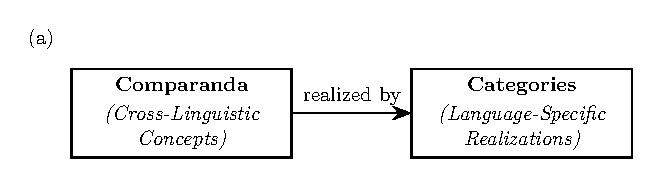
\includegraphics[width=0.95\textwidth]{matrix_figure_v2.pdf}
  \caption{The comparanda--realization mapping. (a) Abstract schema: cross-linguistic comparanda are realized by language-specific categories. (b) Matrix implementation: rows represent comparanda (syntactic functions, semantic targets, discourse roles, categories as comparative concepts), columns represent language-specific forms. Cross-linguistic comparison proceeds row-wise; language-internal analysis proceeds column-wise.}
  \label{fig:matrix}
\end{figure}

\begin{table}[ht]
  \centering
  \caption{Fragment of $M_L$ for English ($L = \mathrm{Eng}$) and Japanese ($L = \mathrm{Jpn}$). Weights are schematic (1 = canonical, 0.5 = secondary, 0 = absent). Rows that target functions list phrasal or constructional realizations; rows that target semantic targets list lexical categories or morphological systems.}
  \label{tab:matrix}
  \small
  \begin{tabular}{p{3.8cm}p{3.6cm}p{1.2cm}p{3.6cm}p{1.2cm}}
    \toprule
    Comparandum $c$ & Realisation in English & $w_{\mathrm{Eng}}(c,\phi)$ & Realisation in Japanese & $w_{\mathrm{Jpn}}(c,\phi)$ \\
    \midrule
    \textsc{determiner}\textsubscript{\Cross} (function) & Determinative phrase & 1.0 & Classifier phrase & 1.0 \\
    \textsc{definiteness}\textsubscript{\Cross} (semantic target) & Determinative & 1.0 & Demonstrative & 0.8 \\
    \textsc{mass/count}\textsubscript{\Cross} (semantic target) & Number morphology & 1.0 & Classifier & 1.0 \\
    \textsc{topic}\textsubscript{\Cross} (discourse role) & Left-peripheral NP + intonation & 0.6 & XP + \textit{wa} & 1.0 \\
    \textsc{focus}\textsubscript{\Cross} (discourse role) & Prosodic prominence & 0.7 & Focus particle + prosody & 1.0 \\
    \textsc{modifier}\textsubscript{\Cross} (function) & Adjective phrase & 0.9 & Relative clause & 1.0 \\
    \bottomrule
  \end{tabular}
\end{table}

Populating $M_L$ follows a simple protocol: define the comparandum, list the diagnostics, score each candidate realization, record provenance, and report inter-coder agreement. Prototypicality rather than exceptionless correlation determines weights: $w_L(c,\phi)=1.0$ marks the canonical exponent of $c$ in $L$ even when systematic exceptions remain (e.g., weak definites and proper names in English both involve systematic divergences from the prototypical definiteness--article pairing). Semantic targets and discourse roles live exclusively in Levels~I and~II, so their rows never contain language-specific meanings but only point to the forms that realize those meanings; language-internal forms occupy only the columns.

Filled matrices for a language sample enable quantifying typological structure: trade-offs (negative correlations among weights), regeneration pathways (diachronic shifts where one category's weight rises as another falls), and naturalization prospects (whether a comparative category like \textsc{noun}\textsubscript{\Cross} shows consistently high, multi-cue weights across diverse families). Sections~\ref{sec:naturalized}--\ref{sec:predictions} develop these analyses. The same matrix supports language-specific work (scanning down a column reveals how \textsc{determinative}\textsubscript{Eng} participates in multiple comparanda) and cross-linguistic comparison (scanning across a row reveals which constructions satisfy \textsc{topic}\textsubscript{\Cross}).


\section{Syntax--semantics hygiene}\label{sec:hygiene}

Semantic targets and discourse roles~-- \textsc{definiteness}\textsubscript{\Cross}, \textsc{specificity}\textsubscript{\Cross}, \textsc{genericity}\textsubscript{\Cross}, \textsc{agentivity}\textsubscript{\Cross}, \textsc{topic}\textsubscript{\Cross}, \textsc{focus}\textsubscript{\Cross}~-- raise a parallel problem. Testing these Level-I comparanda  independently of any particular morphological or syntactic form prevents collapsing semantic targets into their morphosyntactic realizations (examples \ref{ex:definiteness-vs-articlehood} and \ref{ex:specificity-dom}) or treating morphological presence as definitional of semantic categories. The hygiene protocol verifies Level-I comparanda  through behavioural diagnostics independently of any morphosyntactic exponent before recording mappings in $M_L$. This workflow parallels established semantic fieldwork methods that separate meaning probes from morphosyntactic packaging \parencite{Matthewson2004} and mirrors experimental acceptability-judgment practice in psycholinguistics, where interpretations are elicited before forms are analysed \parencite{Cowart1997,Schuetze1996}. Semantic targets and discourse roles are never treated as functions or categories but diagnosed independently and only then linked, via the mapping, to whichever functions and categories express them in $L$.

Defining Level-I comparanda as comparative concepts with operational diagnostics that don't presuppose any single exponent (Rule~B) provides the solution: test the comparandum directly in specific discursive contexts, then record which forms express it in each language.

\subsection{Protocol (excerpt)}\label{subsec:hygiene-protocol}

\begin{exe}
\ex\label{ex:definiteness-cc} \textbf{\textsc{Definiteness}\textsubscript{\Cross}} (identifiability/uniqueness/familiarity): Test whether referents in specific contexts are treated as identifiable through behavioural diagnostics~-- can a referent be picked up anaphorically? Does it trigger uniqueness inferences (\enquote{only X}/bridging)? Is it incompatible with novelty contexts (presentational constructions, existential \textit{there})? These properties cluster but aren't individually necessary; prototypical definiteness shows all three. Do not \emph{infer} \textsc{definiteness}\textsubscript{\Cross} from article categories; articles are realizations, not diagnostics (cf.\ example~\ref{ex:definiteness-vs-articlehood}) \parencite{Lyons1999,Heusinger2011}.

\ex\label{ex:specificity-cc} \textbf{\textsc{Specificity}\textsubscript{\Cross}} (scopal stability): Test whether referents maintain consistent scope across intensional and quantificational environments. Primary diagnostics: Does the referent take wide scope over negation or modals? Does it support choice-function readings (\enquote{speaker has a particular referent in mind})? Secondary diagnostic: Does it remain accessible for subsequent anaphoric reference (noting that this cue overlaps with definiteness)? Avoid treating differential object marking (DOM) as definitional of \textsc{specificity}\textsubscript{\Cross}; DOM is a realization, not a diagnostic \parencite{Enc1991,Heusinger2011}.

\ex\label{ex:genericity-cc} \textbf{\textsc{Genericity}\textsubscript{\Cross}}: Diagnose \textbf{kind-reference} (\textit{Dogs are mammals}: does the NP denote a kind rather than individual dogs?) and \textbf{characterizing predication} (\textit{Dogs bark}: does the sentence attribute a generic property rather than describe a specific event?). These are distinct targets that may align or diverge. Do not conflate bare-noun syntax with \textsc{genericity}\textsubscript{\Cross}, or habitual aspect marking with generic predication~-- form and function dissociate systematically \parencite{KrifkaEtAl1995,Chierchia1998}.

\ex\label{ex:agentivity-cc} \textbf{\textsc{Agentivity}\textsubscript{\Cross}}: Use proto-agent diagnostics \parencite{Dowty1991}: Can the predicate combine with \textit{deliberately}? Does it license \textit{what X did was...} clefts? Does it support control into purpose clauses (\textit{X V-ed in order to...})? Does it entail causation or change-of-state initiated by the argument? Don't simply equate \textsc{agentivity}\textsubscript{\Cross} with subjecthood or nominative case~-- these are formal categories that may or may not align with the semantic target.
\end{exe}

For each Level~I comparandum, we record its \emph{mapping to language-internal forms} in the matrix $M_L$, but we evaluate the semantic or discourse-pragmatic property independently first. This prevents meanings from being reified as (falsely identified with) particular morphosyntactic forms. The examples above (\ref{ex:definiteness-cc}--\ref{ex:agentivity-cc}) function as diagnostic checklists, not as proxies for specific grammatical exponents.

\subsection{Hygiene protocol procedure}\label{subsec:hygiene-procedure}

For each Level~I comparandum $c$ (semantic target or discourse role) and each language $L$, we follow a five-step protocol that enforces independence of diagnostics from morphosyntactic form:

\begin{enumerate}[label=\arabic*., leftmargin=*]
  \item \textbf{Establish diagnostic traction.} Verify that the behavioural tests for $c$ yield consistent judgments in $L$. Select test contexts (minimal pairs, elicited examples, or corpus instances) where the diagnostics should discriminate. If diagnostics fail to yield stable judgments, either refine the tests or recognize that $c$ may not be a relevant comparative concept for $L$.
  
  \item \textbf{Apply diagnostics to contexts.} Test specific NPs, clauses, or discourse contexts using the operational criteria from Section~\ref{subsec:hygiene-protocol}. Score strength of evidence: 0 = diagnostic fails; 1 = weak evidence; 2 = moderate; 3 = strong. Record which diagnostics apply and which don't. This step is conducted \emph{without consulting} morphosyntactic form~-- judgments are based on interpretation, discourse behaviour, and entailment patterns.
  
  \item \textbf{Identify candidate realizations.} Only after completing step~2, survey which morphosyntactic, prosodic, or constructional forms \emph{correlate} with contexts where $c$ was independently diagnosed. Look for forms $\phi$ that appear systematically in contexts scoring high on the diagnostics.
  
  \item \textbf{Score mappings.} For each form $\phi$ that correlates with $c$, assign $w_L(c, \phi)$ based on:
  \begin{itemize}
    \item \textbf{Sensitivity (recall):} Does $\phi$ appear consistently when $c$ is diagnosed? High sensitivity means $\phi$ is a reliable marker.
    \item \textbf{Precision (positive predictive value):} When $\phi$ appears, does it reliably signal $c$, or does $\phi$ serve multiple functions? Note that low precision is expected~-- exponents are typically polyfunctional~-- and should not automatically lower weights (cf.\ Section~\ref{sec:matrix}, weights as prototypicality). A form can be the canonical exponent ($w_L = 1.0$) even when it serves other functions (e.g., English articles mark definiteness but also appear in weak definites and generic frames).
    \item \textbf{Contextual strength:} How robustly does $\phi$ correlate with $c$ across contexts?
  \end{itemize}
  
  \item \textbf{Record provenance and reliability.} Note whether the mapping is uncontroversial (leave $r_L$ unspecified), contested ($r_L$ mandatory, based on inter-coder agreement), or experimentally validated ($r_L$ based on corpus evidence or acceptability judgments). Document which diagnostics were used and how scoring decisions were made.
\end{enumerate}

Crucially, \textbf{step~2 precedes step~3}: we do not infer the presence of Level-I comparanda  from morphological exponents. The protocol prevents circular reasoning and guards against the cluster-reduction and false-universalization errors diagnosed in examples (\ref{ex:definiteness-vs-articlehood}) and (\ref{ex:specificity-dom}). By establishing independent behavioural evidence before examining form, we ensure that mappings in $M_L$ reflect empirical correlation rather than definitional stipulation. Figure~\ref{fig:dag} visualizes this anti-circularity workflow: Stage~1 diagnoses the semantic target from behavioural diagnostics while withholding candidate forms, ensuring statistical independence $(F \perp \hat{\eta}_{\text{Nom}} \mid D, X, B, L)$; Stage~2 then models how the latent target causes observable forms via homeostatic mechanisms.

\begin{figure}[ht]
  \centering
  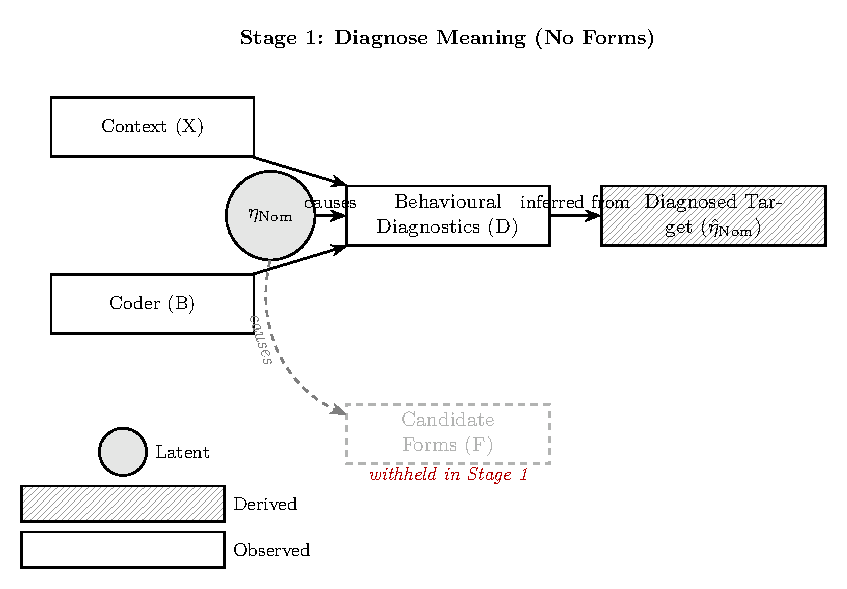
\includegraphics[width=\textwidth]{dag_figure_page1.pdf}

  \vspace{0.5cm}

  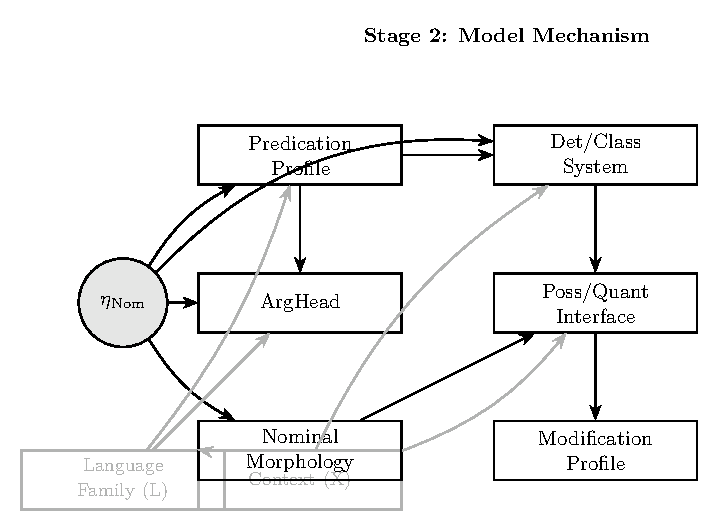
\includegraphics[width=\textwidth]{dag_figure_page2.pdf}
  \caption{The anti-circularity workflow. \textbf{Top:} Stage~1 diagnoses the semantic target ($\hat{\eta}_{\text{Nom}}$) from behavioural diagnostics (D) conditioned on context (X), coder (B), and language family (L), while withholding candidate forms (F) to ensure $(F \perp \hat{\eta}_{\text{Nom}} \mid D, X, B, L)$. \textbf{Bottom:} Stage~2 models how the latent target ($\eta_{\text{Nom}}$) causes observable forms via homeostatic mechanisms, with language family (L) and context (X) as partial pooling and conditioning variables.}
  \label{fig:dag}
\end{figure}

An illustrative failure case shows what happens when hygiene is violated and how the naturalization tests bite. The slogan \enquote{feminine personal names end in /a/} collapses comparandum and exponent: it bundles the Level I target (feminine personal name) with a specific phonological realization (final /a/), leaning on Latin orthography to make the pattern look universal.

Applying the failure modes (Section~\ref{sec:naturalized}):

\begin{enumerate}[label=(\roman*), leftmargin=*]
    \item \textbf{Too fat}: the slogan lumps together unrelated exponents. Feminine names that end in /a/ because of Romance declension suffixes, Turkish vowel harmony, or Arabic templatic vocoids get treated as one “kind,” even though the diagnostics and mechanisms differ.
    \item \textbf{Negative projectibility}: the correlation evaporates outside Indo-European and neighbouring families. Masculine /a/ names (Arabic, Bantu) and feminine names without /a/ (Hebrew, Mandarin, English monosyllables) are plentiful; held-out families invalidate the prediction.
    \item \textbf{Areal/mechanistic failure}: the clustering flows from genealogical inheritance and areal diffusion (Mediterranean Sprachbund, IE suffixal pathways) rather than recurrent cognitive or discourse pressures that would regenerate the pattern independently.
\end{enumerate}

The three-level apparatus handles this cleanly. Define \textsc{feminine personal name}\textsubscript{\Cross} as the comparandum and record how each language realizes it: final low vowel ($w_{\mathrm{IE}} \approx 0.8$), feminine declension suffix ($w_{\mathrm{Lat}} = 1.0$), onomastic formatives ($w_{\mathrm{Sem}} \approx 0.6$), prosodic frames, or no dedicated marking ($w_{\mathrm{Eng}} = 0$ for most names). The diagnostic question (\enquote{Does the name trigger feminine agreement, carry feminine social indexing?}) stays separate from the realization question (\enquote{Which forms signal it?}), satisfying Rule~B and the hygiene protocol. The comparison remains useful within the genealogical/areal zone where the weights are high, but it never meets the criteria for naturalized status because it is too fat, shows negative projectibility, and lacks recurrent mechanisms.

\section{Naturalised comparative concepts}\label{sec:naturalized}
Not all comparative concepts are created equal. Some comparative categories~-- foremost \textsc{noun}\textsubscript{\Cross}~-- show stable patterns across genealogically and areally diverse languages. Nouns\textsubscript{\Cross} canonically serve as argument heads, anchor possessive and quantificational constructions, take characteristic predication patterns, and participate in modification relationships. This clustering isn't random or accidental.

I propose treating such concepts as \emph{naturalized comparative concepts}~-- weak homeostatic property cluster (HPC) kinds operating at the cross-linguistic level (recall Section~\ref{sec:orientation}). For naturalized linguistic concepts, these mechanisms include recurrent cognitive pressures (reference tracking, packaging for quantification), discourse-functional needs (argument realization), and convergent grammaticalization pathways. Section~\ref{subsec:mechanisms} catalogues the full palette.

Not all comparative concepts achieve this status. When concepts fail to stabilize, they can be tagged with explicit failure modes: \emph{too thin} (diagnostics rarely pass across languages), \emph{too fat} (the category overgenerates, lumping together distinct phenomena), \emph{negative} (projectibility metrics underperform statistical thresholds), or \emph{indeterminate} (insufficient data from diverse enough languages to judge).

\subsection{Criteria for naturalization}\label{subsec:naturalization-criteria}
Not all comparative concepts qualify for naturalized status. The bar should be high~-- we want to avoid reinstating the spurious universals we're trying to eliminate. A comparative concept earns promotion when three conditions jointly obtain. First, the diagnostic features have to  cluster reliably across genealogically and areally diverse languages (cross-linguistic property covariation). It's not enough for \textsc{noun}\textsubscript{\Cross}-like patterns to appear in Indo-European; we need evidence from language families with independent evolutionary histories. Second, we have to  specify the cognitive, diachronic, or discourse-functional pressures that explain why the clustering recurs independently (identifiable homeostatic mechanisms). Appeals to \enquote{communicative need} or \enquote{cognitive salience} don't suffice without concrete evidence~-- grammaticalization pathways, acquisition trajectories, discourse-functional asymmetries that can be documented. Third, the posited mechanisms should generate testable predictions about erosion, regeneration, or trade-offs (predictive purchase). If we can't derive falsifiable consequences, the explanation isn't doing real work.

Failure to qualify arises from three warning signs: diagnostics systematically fail in well-described languages outside the European grammatical tradition (suggesting the covariation is an artifact of shared descriptive templates); apparent stability traces to transmitted descriptive frameworks rather than convergent evolution; or no plausible mechanisms can be articulated despite searching. When comparative concepts fail these tests, we tag them with explicit failure modes: \emph{too thin} (diagnostics rarely pass across languages), \emph{too fat} (the category overgenerates, lumping together distinct phenomena), \emph{negative} (projectibility metrics underperform declared thresholds), or \emph{indeterminate} (insufficient data from diverse enough languages to judge).

Reassessment becomes necessary when new evidence challenges previously naturalized status: broader sampling reveals the pattern was genealogically/areally restricted; proposed mechanisms prove inadequate; or predictions fail in held-out data. In such cases, we revise the classification: downgrade from naturalized to instrumental comparative concept, restrict naturalization claims to specific families/areas, or tag with failure modes.

Naturalization is gradient, not binary. \textsc{noun} likely sits near the strong pole: high property covariation across diverse families, multiple reinforcing mechanisms (argument realization, possession, quantification interfaces), clear predictions about paradigm stability and regeneration. \textsc{adjective} occupies a weaker position: the category is absent or diffuse in many well-described languages, fewer convergent grammaticalization pathways, less stable clustering. \textsc{subject}\textsubscript{\Cross} (function) remains contested: definitional circularity (is it a syntactic or semantic notion?), radical variation in alignment systems, unclear whether mechanisms actually converge. The framework provides the test; which concepts pass is an empirical matter.

\subsection{Homeostatic mechanisms: plural levels}\label{subsec:mechanisms}
What actually stabilizes linguistic categories? The answer is plural~-- there's no single mechanism doing all the work \parencite[cf.][]{Miller2021}. Language-internal categories (like NP\textsubscript{Eng} or construct state\textsubscript{Heb}) draw on community-specific mechanisms: cognitively, acquisition biases and processing constraints (children learning English converge on the NP early and consistently); socially, community norms, prescriptive regimes, and interactional routines (standard grammars codify noun paradigms, schools drill them, style guides police their use); materially, literacy and orthography (written standards, dictionaries, grammatical treatises); diachronically, regenerative pathways (grammaticalization, reanalysis, analogy) that rebuild eroded exponents, with erosion-resistance from paradigmatic pressure and frequency-driven entrenchment.

Naturalised comparative concepts exhibit homeostasis through recurrent but independent mechanisms operating across unrelated languages: cognitive-functional pressures (reference tracking, individuation, quantificational packaging) driven by stable discourse demands; discourse-adaptive asymmetries (arguments versus predicates, topics versus comments) from information structure; convergent grammaticalization routes (demonstratives becoming articles, measure terms becoming classifiers, relational nouns becoming adpositions). Areal diffusion can amplify these patterns within contact zones.

The HPC claim is modest: each kind is stabilized by some specifiable mix of these forces, to be discovered through empirical investigation. The causal profile differs by level~-- community-bound for language-internal categories, globally recurrent for naturalized comparative concepts~-- but both satisfy the homeostatic template.

\section{Interlude: what eyes buy us}\label{sec:eyes}
Consider camera eyes. Vertebrates and cephalopods (octopuses, squid) both have them, complete with lens, retina, and iris. But  these lineages diverged over 500 million years ago~-- their eyes are analogous organs, not inherited from a common ancestor with a camera eye. The puzzle: how can the \enquote{same} structure appear independently?

The answer lies in \emph{character-identity mechanisms} (CIMs)~-- developmental processes in gene-regulatory networks that maintain structural sameness across evolutionary time and convergent evolution \parencite{ShubinTabinCarroll2009,Wagner2014,DiFriscoLoveWagner2020}. Even though vertebrate and cephalopod eyes evolved separately, they recruit conserved genetic toolkits (like Pax6 genes) that bias development toward similar functional solutions. CIMs don't specify essences; they describe the processes that keep a biological structure recognizable despite variation.

For linguistic typology, I propose analogous \emph{character-identity mechanisms for language} (CIM-L) that maintain category behaviour through diachronic change and cross-linguistic convergence:


\begin{description}
    \item[Invariance] Stable mapping from discourse-functional demands (identifiability, individuation, possession, quantification) to privileged morphosyntactic slots. Nouns reliably serve as argument heads, anchor possessive constructions, and interface with quantification~-- this mapping persists even as specific morphology changes.

    \item[Cohesion] Paradigmatic and selectional pressures that penalize drift. Once a language establishes determinative or classifier systems, case or construct morphologies, and modification profiles, these co-adapted traits resist being pulled apart. Changing one element (say, losing case) creates pressure to compensate elsewhere (developing stricter word order).

    \item[Regeneration] Recurrent diachronic sources that rebuild eroded exponents. When articles weaken, languages reliably find new sources: demonstratives grammaticalize into definite markers (deixis $\to$ articles), measure terms become classifiers (measure/class terms $\to$ classifiers), verbs nominalize to create new argument-taking categories (nominalizers $\to$ nouns). The pathways recur because functional pressures remain stable.
\end{description}

These mechanisms explain why \textsc{noun} behaves as a stable HPC across genealogically diverse languages without positing universals or essences. Just as camera eyes reflect convergent solutions to stable functional demands (detecting light, focusing images), noun-like categories reflect convergent solutions to stable discourse demands (picking out entities, tracking reference, anchoring modification). The stability is real, but it's maintained by mechanisms, not mandated by innate categories or semantic primitives.

\section{From labels to measurement}\label{sec:measurement}
Traditional typology trades in binary tallies: language X \term{has} adjectives or it doesn't, nouns \term{mark} number or they don't. This forces clean boundaries where the data show gradients and partial patterns. The three-level mapping (Section~\ref{sec:matrix}) and the hygiene protocol (Section~\ref{sec:hygiene}) provide the foundation for something better: explicit measurement models with declared performance thresholds.

The first move is to replace binary category labels with \emph{latent variables} that represent the degree to which a language instantiates a given comparative concept. For \textsc{nominality}\textsubscript{\Cross}, define a vector of observable diagnostics:
\[
  \begin{aligned}
  \mathbf{n}_L = \big\langle
     &\text{ArgHead},\ \text{Poss/Quant Interface},\ \text{NomMorph},\\
     &\text{Det/Class System},\ \text{Predication Profile},\ \text{Modification Profile}
  \big\rangle.
  \end{aligned}
\]
To do this, we replace simple scores with a statistical model that estimates the latent \enquote{\textsc{nominality}\textsubscript{\Cross}} while fully quantifying our measurement uncertainty. We fit a multilevel ordinal IRT model to the diagnostic ratings. This model is \enquote{multilevel} because it accounts for shared history by grouping related languages (via partial pooling by family/area), and it explicitly estimates the varying informativeness of each diagnostic test as well as \enquote{coder effects} (differences between researchers). Instead of a single score, the model's output is a full posterior distribution (a range of plausible values) for each language's \textsc{nominality}\textsubscript{\Cross} parameter (possibly multidimensional). Finally, we validate the model's adequacy using posterior predictive checks (checking if the model can generate realistic-looking data) before using these summaries descriptively.

The same logic extends to other comparative concepts: \textsc{adjectivality}\textsubscript{\Cross} (modification, predication, gradability, comparison), \textsc{verbiness}\textsubscript{\Cross} (predicate-head privileges, tense-aspect-mood morphology, argument structure). Each gets its own diagnostic vector and measurement model. Semantic targets are tested independently (Section~\ref{sec:hygiene}) and linked to categories only via the observed mappings in the matrix $M_L$ (Rule~B).

Naturalization candidates are evaluated against declared projectibility metrics (ROC-AUC for classifiers, macro-F1 for multi-class prediction) with thresholds that have to  hold in held-out test data before promotion. Failure to meet these thresholds triggers explicit failure modes: too thin, too fat, negative, or indeterminate. The framework thus builds measurement discipline into the theoretical machinery.

\section{A reproducible codebook (excerpt)}\label{sec:codebook}
Measurement discipline requires operational codebooks: explicit diagnostics, decision rules, reliability checks, and provenance tracking for every comparandum (function, target, role) and every category. Below are four illustrative entries showing the required structure. A full implementation would provide this level of detail for every row in the comparanda inventory and every category under evaluation.


\begin{exe}
\ex \textbf{Comparative category: \textsc{noun}\textsubscript{\Cross}.} Diagnostics: argument-head privileges; possessive/quantificational interfaces; nominal morphology; predication and modification profiles. Record which language-internal categories realize it and how strongly (e.g., \textsc{noun}\textsubscript{Eng}, \textsc{classifier}\textsubscript{Tha}) and track the evidence supporting each weight.
\ex \textbf{Syntactic function: \textsc{determiner}\textsubscript{\Cross}.} Diagnostics: dedicated articles (definite/indefinite); demonstratives in selectional use (not just deictic); classifier/measure structures licensing numeral combination; distribution of bare NPs in argument positions (\textsc{subject}\textsubscript{\Cross}, \textsc{object}\textsubscript{\Cross}). Code gradient strength 0--3 (absent $\to$ fully grammaticalized). Record specific exponents (morphemes, constructions) and genealogical provenance (inherited, innovated, contact-induced).

\ex \textbf{Semantic target: \textsc{definiteness}\textsubscript{\Cross}.} Diagnostics: anaphoric uptake (can the referent be picked up by pronouns or repeated definites in subsequent discourse?); uniqueness and bridging (does the expression trigger \enquote{only one} inferences or support part-whole bridging?); anti-novelty contexts (is the expression blocked in presentational or existential constructions where the referent has to be new?). Code strength of evidence on a gradient scale. Do \emph{not} use presence of articles as a diagnostic criterion~-- that would bake in the very conflation we're trying to avoid.

\ex \textbf{Discourse role: \textsc{topic}\textsubscript{\Cross}.} Diagnostics: sentence-initial position preference; aboutness tests (\enquote{As for X, \dots}); persistence across discourse spans; compatibility with focus operators. Code strength 0--3. Record whether topic is marked morphologically (particles, case), positionally (preverbal/post-verbal), or both. Note interaction with \textsc{subject}\textsubscript{\Cross} function and information structure.
\end{exe}

A valid implementation requires guarding against researcher degrees of freedom. Diagnostics should be preregistered before examining cross-linguistic data; post-hoc selection capitalizes on chance. Weight-assignment criteria (when does a realization count as 0.5 vs 0.7?) have to  be established via training data and inter-rater agreement; thresholds chosen to maximize apparent clustering are circular. Inter-rater reliability should reach Cohen's $\kappa > 0.7$ on comparandum--category mappings, with disagreements resolved via pre-specified decision rules rather than negotiation toward desired outcomes. Cross-validation requires reserving a subset of languages (e.g., 20\%) for held-out testing; patterns that fail to replicate in unseen data indicate overfitting. Finally, coding needs to stratify by genealogy, area, and literacy availability (Section~\ref{sec:predictions}); ignoring these risks attributing mechanism-driven patterns to spurious correlates. These precautions sketch an implementation blueprint: the present paper confines itself to the theoretical scaffolding while pointing to the statistical toolkit future empirical work needs to mobilize. The apparatus is designed for iterative refinement: initial codings reveal where diagnostics fail, prompting revision of the comparative concept or recognition that it lacks naturalized status. The specific metrics and models mentioned (Cohen's $\kappa$, factor analysis, IRT) are illustrative examples that operationalize the constraints, not mandatory choices; alternative methods meeting the same standards are equally admissible.

\section{Predictions and risk}\label{sec:predictions}
The three-level mapping (Section~\ref{sec:matrix}), the hygiene protocol (Section~\ref{sec:hygiene}), and the homeostatic mechanisms catalogue (Section~\ref{subsec:mechanisms}) collectively yield five testable cross-linguistic predictions. Each specifies a success criterion with declared thresholds. The statistical tests listed (Spearman correlation, macro-F1, hazard ratios, ROC-AUC) are illustrative implementations; any method that operationalizes the same predictions with transparent diagnostics is admissible.

\begin{enumerate}
    \item \textbf{Trade-off (syntactic functions + semantic targets)}: strength of classifier systems negatively correlates with obligatory number morphology on common nouns. Classifiers realize both \textsc{determiner}\textsubscript{\Cross} and \textsc{mass/count}\textsubscript{\Cross}; number morphology realizes \textsc{mass/count}\textsubscript{\Cross} independently. Success criterion: Spearman $\rho \leq -0.4$ (95\% credible interval excluding zero) on held-out genealogical strata.
    \item \textbf{N--A separation (syntactic functions)}: strong possessive/construct morphology predicts sharper \textsc{noun}\textsubscript{\Cross}--\textsc{adjective}\textsubscript{\Cross} predication splits. Success criterion: mixed-effects logistic models yielding macro-F1 $\geq 0.70$ when predicting adjective-like behaviour from construct diagnostics.
    \item \textbf{Regeneration (syntactic functions)}: weakening of article systems for \textsc{determiner}\textsubscript{\Cross} is followed by increased use of nominalisers and possessive frames for the same function. Success criterion: hazard ratios $>1.5$ in survival models tracking \textsc{determiner}\textsubscript{\Cross} erosion vs. nominaliser uptake.
    \item \textbf{Semantics decoupling (semantic targets)}: languages without articles nevertheless show strong \textsc{definiteness}\textsubscript{\Cross} effects; correlation between article presence and \textsc{definiteness}\textsubscript{\Cross} weakens once hygiene is enforced. Success criterion: ROC-AUC $\geq 0.75$ for \textsc{definiteness}\textsubscript{\Cross} diagnostics in article-less languages.
    \item \textbf{Specificity non-identity (semantic targets)}: presence of DOM improves \emph{detectability} of \textsc{specificity}\textsubscript{\Cross} but is neither necessary nor sufficient for it; wide-scope diagnostics sometimes diverge from DOM. Success criterion: false-negative rate $\leq 0.20$ for \textsc{specificity}\textsubscript{\Cross} detection in families lacking DOM.
\end{enumerate}

Threshold values (e.g., $\rho \leq -0.4$, F1 $\geq 0.70$) are provisional benchmarks provided impressionistically; empirical work should recalibrate them via model comparison and posterior predictive checks. Each prediction is coupled to a declared diagnostic threshold so that projectibility is falsifiable: values outside the bands signal that naturalization has failed and help diagnose whether covariation is too thin, mechanisms too weak/too fat, or projection unreliable. (Spearman's $\rho$ is a rank correlation, macro-F1 a class-averaged F1 score, hazard ratios quantify relative event rates in survival models, while ROC-AUC and false-negative rate summarise classifier performance.)

These tests represent pragmatic, illustrative checks on the framework's predictions. A better, fully integrated approach would frame these hypotheses as parameters within the unified generative model proposed in Section~\ref{sec:measurement}, for example, by modelling correlation trade-offs as covariance parameters to be estimated, rather than as simple post-hoc correlations.

Literate traditions introduce additional stabilizers~-- orthographic standards, grammars, dictionaries, and metalinguistic policing~-- that can amplify or arrest these trajectories. Oral settings rely more heavily on cognitive and interactional mechanisms, so regeneration and erosion may proceed differently across the predictions above. Any measurement agenda has to therefore stratify by the availability of literacy-driven mechanisms when estimating homeostatic strength.

\section{Worked illustrations}\label{sec:illustrations}
The recurring claim that some languages lack adjectives is traditionally treated as evidence against universal lexical categories: if Language X lacks an adjective category, it has to lack the property-modification function entirely, therefore adjectives are not universal and typological variation is radical.

The present framework dissolves this debate by separating levels. We distinguish the \textsc{modifier}\textsubscript{\Cross} function from the \textsc{adjective}\textsubscript{$L$} category, then populate $M_L(\textsc{modifier}\textsubscript{\Cross}, k)$ for the language in question. A typical profile might show: Relative clause constructions (1.0), Property nouns (0.7), Stative verbs in attributive frames (0.5), \textsc{adjective}\textsubscript{$L$} category (0). The \textsc{modifier}\textsubscript{\Cross} function is realized; the \textsc{adjective}\textsubscript{$L$} category is absent.

The framework generates a testable prediction: languages lacking a dedicated \textsc{adjective}\textsubscript{$L$} category should exhibit compensatory elaboration~-- more complex relative-clause syntax, richer nominal modification paradigms, or increased use of stative predicates in attributive position \parencite{Dixon2010,Croft2001}.

Instead of a universal-vs-variation debate about adjectives, we predict the \emph{profile} of modification strategies. Cross-linguistic comparison proceeds by function (row-wise: how is \textsc{modifier}\textsubscript{\Cross} realized?), while language-internal analysis tracks categories (column-wise: which comparanda does this category realize?). Apparent counterexamples to universals become expected patterns once levels are distinguished.

A second illustration concerns numeral--noun ordering correlations. Typological generalizations like \enquote{numeral-noun order correlates with adjective-noun order} often conflate comparanda and categories. When we separate them, clearer patterns emerge. The relevant syntactic functions are \textsc{quantification interface}\textsubscript{\Cross} and \textsc{modifier}\textsubscript{\Cross}; the categories realizing them vary (numerals, classifiers, adjectives, relative clauses). Re-coding the data by function rather than category label weakens some reported effect sizes while revealing new conditioning factors~-- for instance, the presence of classifier systems predicts different ordering patterns than bare numeral-noun combinations. What looked like a direct morpheme-order correlation turns out to reflect deeper functional packaging strategies.

The hygiene protocol's payoff is clearest in the definiteness domain. Traditional surveys equate \textsc{definiteness}\textsubscript{\Cross} with articles: languages \term{have} \textsc{definiteness}\textsubscript{\Cross} if they grammaticalize \textit{the}/\textit{a}-type morphemes. But when we test \textsc{definiteness}\textsubscript{\Cross} independently using discourse diagnostics (anaphoric uptake, uniqueness, anti-novelty), the semantic target is still clearly present in languages lacking article systems \parencite{Lyons1999,Matthewson2004}.

Salish languages, for instance, show strong \textsc{definiteness}\textsubscript{\Cross} effects in referential behaviour despite having no definite articles. Semantic targets survive category turnover~-- forms come and go (articles grammaticalize, erode, get replaced), but the functional pressures driving identifiability marking remain stable.

\section{Threats and replies}\label{sec:threats}
A first objection concerns languages with flexible lexical categories. What about Salish or Riau Indonesian, where word-class boundaries are notoriously fluid? The framework handles this gracefully. Boundary crispness is itself a measurable property~-- some languages show sharp \textsc{category}\textsubscript{$L$} distinctions, others show gradient membership.

Latent variable models (Section~\ref{sec:measurement}) recover the functional clustering even when morphological diagnostics give weak signals. The matrix simply records which categories realize which comparanda (functions, targets, roles) with what weights; languages with flexible classes will show distributed weights across multiple categories rather than sharp 0/1 contrasts. This is descriptively accurate, not a defect. Crucially, semantic targets and discourse roles can still be measured independently even when \textsc{category}\textsubscript{$L$} boundaries blur~-- \textsc{definiteness}\textsubscript{\Cross} diagnostics and \textsc{topic}\textsubscript{\Cross} tests don't depend on crisp lexical class membership.

A second question asks how we distinguish genealogical inheritance (homology) from independent convergent evolution (analogy) versus contact-induced diffusion. All three produce cross-linguistic similarity, but the mechanisms differ.

The framework handles this by tracking genealogical identity separately from comparandum similarity. When coding a language, we record provenance: is this exponent inherited from a documented proto-form, innovated within the attested history of the language, or borrowed from a contact neighbor? Areal patterns get flagged explicitly. Both genealogical and comparandum patterns are reported; the distinction matters for testing which homeostatic mechanisms are active (inherited paradigms versus recurrent grammaticalization versus diffusion).

Inter-coder reliability is non-negotiable for measurement validity. The codebook (Section~\ref{sec:codebook}) specifies decision rules, provenance fields, and reliability checks for every diagnostic. When coders disagree, adjudication proceeds at the comparandum level (function/target/role) using operational tests, not by negotiating category labels.

For example, if Coder A and Coder B disagree on whether an element is a \textsc{determinative}\textsubscript{$L$}, the resolution protocol asks: does it realize \textsc{determiner}\textsubscript{\Cross}? Does it encode \textsc{definiteness}\textsubscript{\Cross}? Does it participate in selectional restrictions? Does it combine with numerals? The diagnostics settle the question, not intuitions about what \enquote{feels like} a determiner.

The proposal demands substantial coding effort~-- diagnostic batteries applied across dozens of languages, each requiring expertise and careful adjudication. This is labour-intensive, though this scaling challenge can be substantially mitigated by modern tools. Large Language Models (LLMs), for example, can be leveraged to bootstrap this process, applying the diagnostic codebook (\S\ref{sec:codebook}) to corpora at scale.

Crucially, this does not replace expert adjudication but reframes it as a task of validation. The LLM's output has to be treated as that of a research assistant, subject to the same rigorous inter-rater reliability checks (e.g., Cohen's $\kappa > 0.7$) and error analysis as any human-generated coding. This approach makes the required scaling tractable, and the framework's explicit \enquote{coder effects} parameter (see \S\ref{sec:measurement}) is designed to model and manage such rater-specific variation, whether human or not.

This is not unprecedented: existing typological databases (WALS, Grambank, APiCS) demonstrate that systematic cross-linguistic coding is tractable when protocols are explicit and inter-rater reliability is monitored. The present framework reduces measurement error by separating levels (syntactic functions, semantic targets, discourse roles, and language-specific categories) and using gradient scores rather than forcing binary tallies.

Pilot studies on 10--15 well-described languages can establish feasibility before scaling. The apparatus is designed for iterative refinement: initial codings reveal where diagnostics fail, prompting revision of the comparative concept or recognition that it lacks naturalized status.

What would force us to reassess and potentially withdraw naturalized status? Failure on any of the three criteria from Section~\ref{subsec:naturalization-criteria}: diagnostics systematically fail in genealogically diverse languages; proposed homeostatic mechanisms dissolve under scrutiny; or predictions fail in held-out data. Such disconfirmation reveals that the concept was misclassified initially (appeared naturalized within a limited sample but lacks genuine cross-linguistic stability) or requires scope restriction (naturalized within certain families/areas but not globally).

A related worry concerns circularity. Do the diagnostics for, say, nominality presuppose what counts as a noun, creating a circular validation? The hygiene protocol blocks this: diagnostics are framed as independent operational tests (Does this element serve as argument head? Does it anchor possessive constructions? Does it combine with determiners/classifiers?) rather than as checks for category membership.

A language may score high on some diagnostics, low on others; the matrix records the profile without forcing a binary noun/not-noun decision. When diagnostics cluster strongly, that empirical covariation \emph{warrants} positing a naturalized category; when they scatter, the concept remains useful for comparison but loses HPC status. The test is whether independent researchers, applying the operational criteria, converge on similar profiles~-- a matter for inter-coder reliability studies, not a priori stipulation.

Finally, does promoting comparative concepts to naturalized status reintroduce universals through the back door? No, for four reasons.

First, naturalization is \emph{gradient} (strong/weak/contested), not binary; universals do not admit degrees. Second, naturalization is \emph{empirically defeasible}: demotion criteria in Section~\ref{subsec:naturalization-criteria} specify conditions under which a concept loses naturalized status; universals are not revisable in light of counterexamples.

Third, cross-linguistic stability is explained by \emph{independent convergent mechanisms}, not shared essences: Japanese and English both exhibit \textsc{noun}\textsubscript{\Cross}-like patterns, but these are maintained by distinct community-specific mechanisms that happen to arise from recurrent pressures (reference tracking, individuation). Fourth, a naturalized concept may be strong in some language families and absent or diffuse in others (e.g., \textit{adjective} shows weak naturalization, present in Indo-European but marginal in many other families). This is convergent evolution, not universality. The framework predicts which concepts will show high versus low naturalization strength, whereas universalist approaches assume uniform presence or categorical absence.

\section{Conclusion}\label{sec:conclusion}
The solution rests on three pillars: comparanda discipline (explicit mappings $M_L(c,\phi)$ separating cross-linguistic functions from language-internal categories); semantics hygiene (testing meanings independently of morphosyntactic forms via behavioural diagnostics); and measurement accountability (latent variable models with declared performance thresholds, making naturalization empirically defeasible).

The framework treats language-internal categories as genuine homeostatic property clusters: community-specific kinds maintained by cognitive, social, material, and diachronic mechanisms. A few comparative concepts~-- \textsc{noun} foremost among them~-- may qualify as \emph{naturalized}: weak HPCs sustained by recurrent but independent mechanisms across unrelated languages. These aren't universals (they're gradient, defeasible, and maintained by convergent evolution rather than shared essences), but they're not arbitrary analyst constructs either. The evidence for naturalization comes from the predictions in Section~\ref{sec:predictions}: trade-offs, regeneration pathways, compensatory elaboration, and decoupling of semantics from morphology.

The result is a typology with fewer spurious universals, clearer explanations grounded in specifiable mechanisms, and replicable paths from description to prediction. The three-level mapping, the hygiene protocol, and the measurement models provide an implementation blueprint; the formal specification in \texttt{src/typology.py} offers an auditable encoding of the theoretical commitments. What remains is empirical work: coding languages, testing predictions, refining diagnostics, and discovering which comparative concepts earn naturalized status and which dissolve under scrutiny.

\clearpage
\printbibliography

\end{document}
